\documentclass[12pt,a4paper]{article}

\usepackage{times}
\usepackage[T1]{fontenc}
\usepackage{graphicx}
\usepackage{subfig}
\usepackage{caption}
\usepackage{epsfig}
\usepackage{epstopdf}
\usepackage{fancyhdr}
\usepackage[dvipsnames]{color}
\usepackage{hyperref}
\usepackage{amsmath}
\usepackage{multicol}
% \usepackage[slovak]{babel}
\usepackage{float}

\usepackage[backend=bibtex, style=numeric, citestyle=authoryear, sorting=none]{biblatex}
% \addbibresource{sources.bib}
\renewcommand*{\nameyeardelim}{\addcomma\addspace}

\textwidth = 170.0mm
\textheight = 246.0mm

\topskip=5mm
\topmargin=0mm
\evensidemargin=-5.4mm
\oddsidemargin=-5.4mm
\headheight=14pt
\headsep=5mm

\parindent=0mm
\parskip  =2mm

\pagestyle{fancy}

\fancyfoot[C]{}

\voffset=-1.25cm
% \pagenumbering{arabic}
% \setcounter{page}{1}
\pagestyle{plain}
\headheight=15pt

%\definecolor{mygray}{cmyk}{0,0,0,0.4}
\definecolor{mygray}{gray}{0.5}

\rhead{\textcolor{mygray}{\fontsize{10}{12}\selectfont DEEP LEARNING FOR COMPUTER VISION}}
\renewcommand{\headrule}{{\color{mygray}%
       \hrule width\headwidth height\headrulewidth \vskip-\headrulewidth}
}%renewcommand headrule

\renewcommand\textfraction{.02}
\renewcommand\floatpagefraction{.98}

% for rule under section heading
\newcommand {\sectionrule}{\vskip -0.9 cm
\color {mygray} \rule [0 cm] {17 cm}{0.1 mm} \color {black}}

%%%%%%%%%%%%% START %%%%%%%%%%%%% 
\date{}

\title{HW1 \\ Classification Task on Cifar-10}

\author{Bc. Martin Vozár}

\begin{document}
\maketitle
% \thispagestyle{fancy}

\section{Approach}
\sectionrule

The assignment proposes working with a standardized dataset on a 
straight-forward task and encourages trying multiples of different
configurations. First step in the process should be finding and choosing
appropriate configuration as a baseline.

For those purposes, we developed a handy framework for setup
of various configurations, similar to hyperparameter optimization
(see \emph{configs/*} for more details).
We are plotting $\text{torch.nn.CrossEntropyLoss}$ as our loss function,
and accuracy as our metric for both $\text{Training}$ and $\text{Test set}$.
Plots are made on a $\text{log}/\text{log}$
scale, as it allows easier interpretation and detections of potential
issues (see \emph{log2png.py} for more details).

After finding the baseline, we further explore chosen configuration
in effort to maximize accuracy.

The code was ran in \emph{conda} environment on \emph{Ubuntu 22.04} using
a single \emph{NVIDIA GTX 1070 Ti}. The code is adapted to function
without issues on CPU as well, albeit quite slower in comparison.

\section{Preliminary exploration}
\sectionrule

In this stage, we are mostly comparing different optimizers 
(SGD, SGD with Momentum=0.96, Adam, and AdamW) with
different learning rates. We are using defaultvalue for batch size
(128), and minimal data augmentation (RandomFlipVertical(p=0.5),
RandomFlipHorizontal(p=0.5)). We are using LeakyReLU as the default
activation function.

During optimization we perform gradient clipping and use
weight decay argument for all optimizers as means of regularization,
as well as nn.Dropout(p=0.3) as the very first layer. 

For each plot, we plot horizontal lines for maximum Test Accuracy
and minimum Test Loss in the respective plots.

\subsection{Naive - FFCN}

As a first choice meant to calibrate the general setup of
different optimizers, as well as gaining intuition for necessary
complexity of further examined Neural Networks, we tested a simple
FCNN (further as a nickname - Naive).

Iteratively, we tuned individua learning rates for each optimizer
(as their behaviour varied quite a bit) as well as the Network
width and depth. 

Plotted are results for a Network:
\begin{itemize}
  \item nn.Linear(3072, 256)
  \item (nn.Linear(256, 256)) * 8
  \item nn.Linear(256, num\_classes)
\end{itemize}
with activation function after each but last layer. Torch
implementation of CrossEntropyLoss allows us to omit applying
Softmax on output layer, as well as one-hot encoding on the
labels.

\begin{figure}[H]
  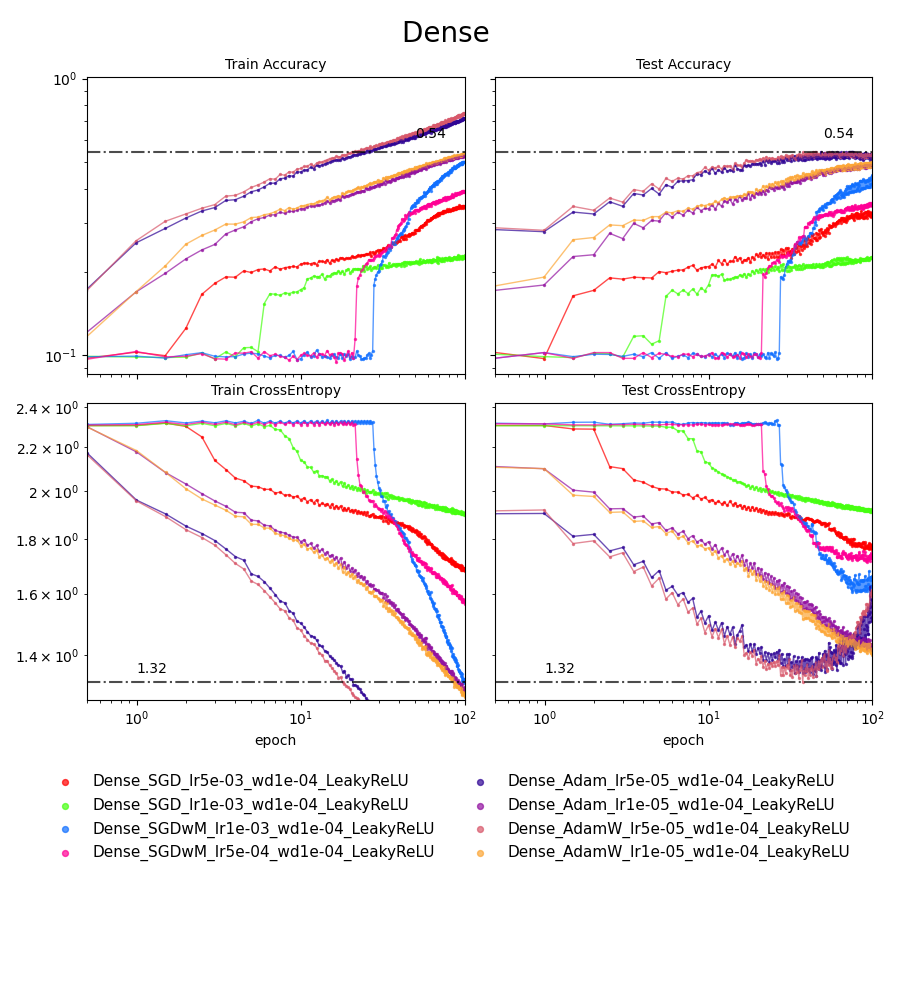
\includegraphics[width=\textwidth, trim={0, 3.5cm, 0, 0}, clip]{../logsDense.png}
  \caption{Plot of results of the preliminary exploration of FCNN
  architecture.}
\end{figure}

\newpage

In those results, we clearly observe examples of overfitting in
most of the runs.

The second thing we can observe is a stagnation of SGD optimization.
Somewhat surprisingly, variants using Momentum stagnated for longer
period of time before proceeding to overfit.
However, this could be acredited to other factors, e.g.
specific initialization of weights.

\subsection{Convolutional Encoder}

We tested a few different variants of Convolutional Encoder. All variants
consisted of blocks of (nn.Conv2d layers, nn.MaxPool2d) and a final
nn.Linear layer at the end. Variables were strides of the convolutions
and number of blocks.

Plotted is the variant which achieved the target accuracy of 70\%
using SGD with Momentum as optimizer. We used this variant in the
following architectures as the final encoding component.

\begin{figure}[H]
  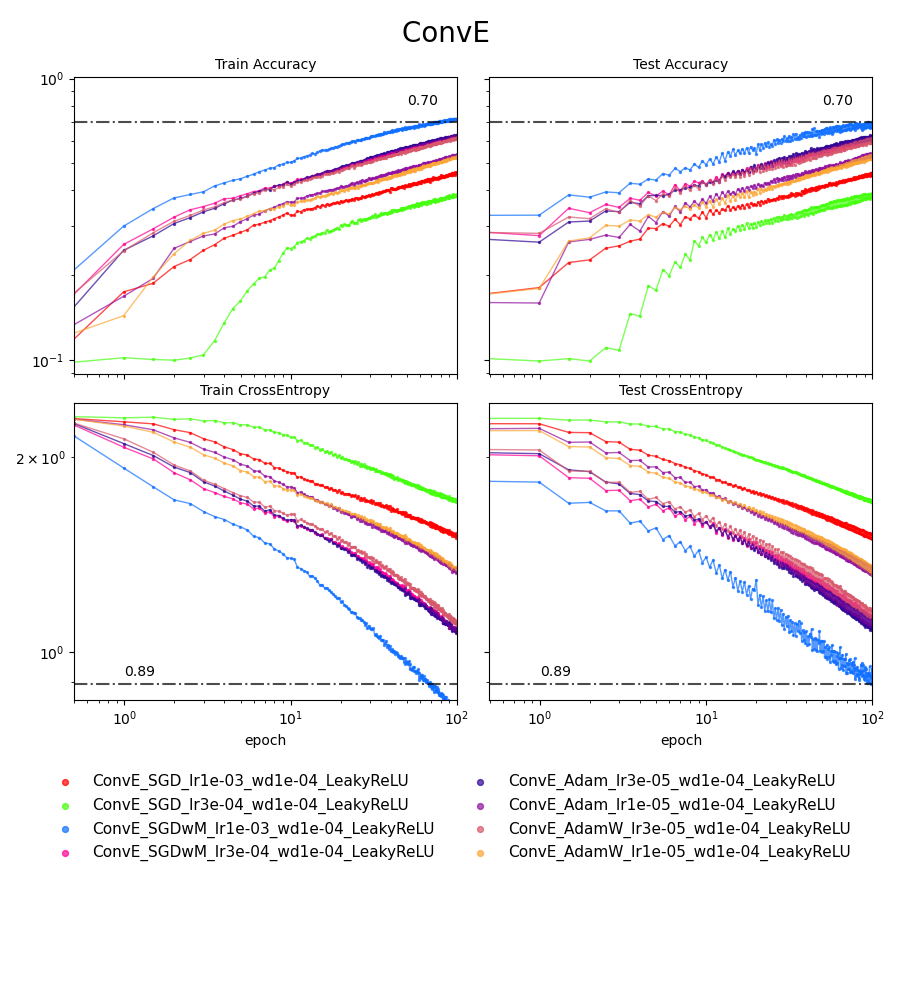
\includegraphics[width=\textwidth, trim={0, 3.5cm, 0, 0}, clip]{../logsConvE.png}
  \caption{Plot of results of the preliminary exploration of ConvEncoder
  architecture.}
\end{figure}

\newpage

\subsection{Residual Convolutional Encoder}

Drawing inspiration from ResNet architecture, we implemented a
basic adaptation of the principle.

The basic idea of the architecture:
\begin{itemize}
  \item nn.Conv2d(in\_channel=3, out\_channels=16, kernel\_size=1, stride=1)
  \item N x ResBlock
  \item ConvEncoder
\end{itemize}

The first layer expands the number of channels to a set number,
which then remains unchanged passing through the ResBlocks. Finally,
Convolutional Encoder (adapted to also handle in\_channels different
from original images) outputs the logits.

From multiple tried and tested variants of ResBlock, we settled on definition:
\begin{itemize}
  \item input x
  \item z = nn.Conv2d(in\_channels=16, out\_channels=32)(x)
  \item z = nn.BatchNorm2d(num\_features=32)(z)
  \item z = activation(z)
  \item z = nn.Conv2d(in\_channels=32, out\_channels=16)(z)
  \item z = nn.BatchNowm2d(num\_features=16)(z)
  \item output x = x + z
\end{itemize}

It has been argued (source: some internet forum) that using Dropout and 
BatchNorm at the same time
can lead to issues during the training. However, we have not encountered
(or at least identified) any artifacts, and BatchNorm can boost
convergene and regularization.

Various number of in/out\_channels were tested and those values were
chosed as a reasonable compormise between convergence speed
and potential for accuracy.
We used kernel\_size=3, stride=1, padding=1 bias=False in both 
convolutional layers.

For this configuration, we first tested for N=4 (\# of ResBlocks)
to find the best performing configuration. Then, we varied the
depth of the Network, as well as other parameters.

In Figure 3., we observe an increase to accuracy 77\%. The most accurate
Network seems to have already plateaued, signifying approaching limit
of this configuration.

Interpreting the behaviour of the optimizers, we select SGD with Momentum
and AdamW for further examination. We observe similar behvaiour as with
ConvEncoder. To explore further, we vary the num\_blocks in the RN
architecture, and vary learning rates and weight decay with selected
optimizers.

\begin{figure}[H]
  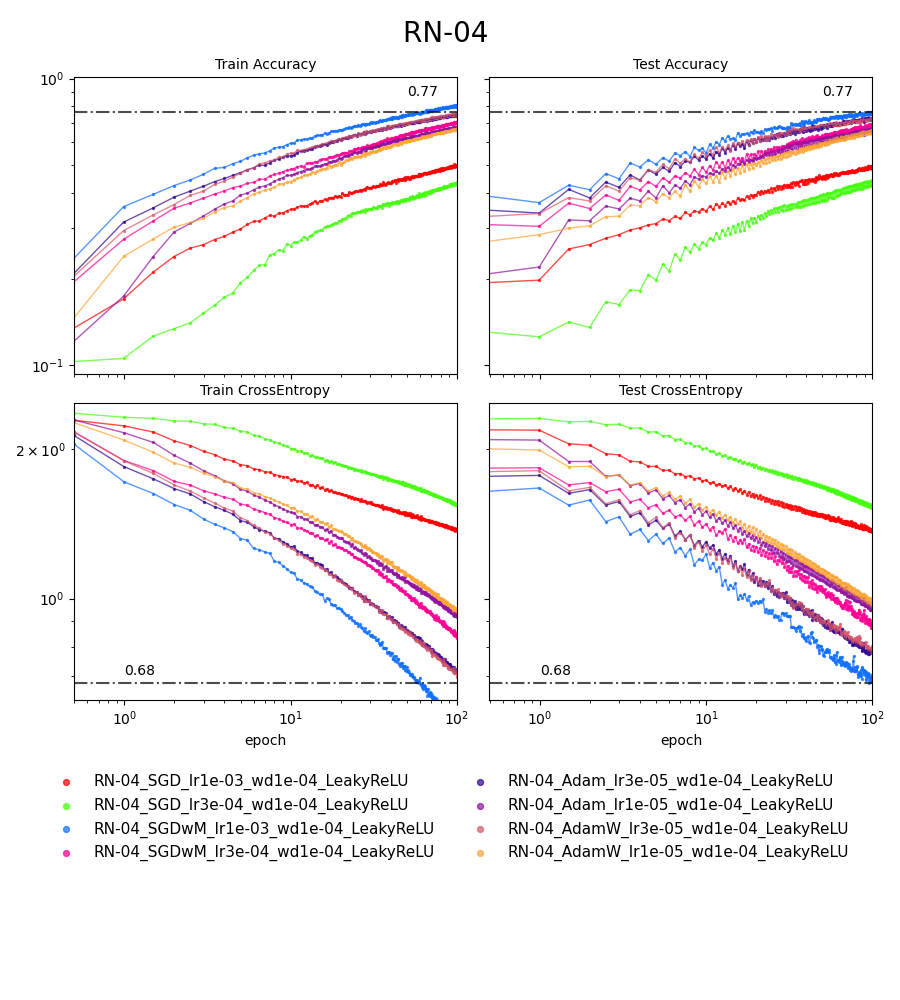
\includegraphics[width=\textwidth, trim={0, 3.5cm, 0, 0}, clip]{../logsRN-04.png}
  \caption{Plot of results of the preliminary exploration of RN04 with ConvEncoder
  architecture.}
\end{figure}

\section{Depth and Learning Rate of RN variants exploration}
\sectionrule

\end{document}

 
